\documentclass{NJUSTThesis}

\usepackage{amsmath} % 数学功能的宏包
%\usepackage{unicode-math} % 设置数学字体Unicode宏包
\usepackage[hidelinks]{hyperref} % 超链接
\usepackage{booktabs} % 提供三线表功能
\usepackage{subcaption} % 提供子图功能,不能使用subfigure宏包
\usepackage{appendix} % 附录功能

\hypersetup{
  bookmarksnumbered=true, % 在书签中显示章节编号
  bookmarksopen=true, % 展开书签
}

% 设置数学字体为 XITS Math,类罗马字体风格,需要先安装该字体
% \setmathfont{Times New Roman} % 设置数学字体为新罗马字体
%\setmathfont{XITS Math}
\usepackage[subscriptcorrection,slantedGreek,nofontinfo]{mtpro2}

%\everymath{\displaystyle} % 行内公式为展示模式
 
\addbibresource[location=local]{reference.bib}

\njustsetup{
  info = {
  % 标题
    title = {
      zh = {南京理工大学本科\\学士学位论文\LaTeX{}模板},
      en ={Nanjing University of Science \& Technology \\ \LaTeX{} Template},
    },
    author = {
      zh = {书雪},
      en = {Xue Shu}, % 作者姓名
    },
    tutor = {
      school/zh = {书雪},
      external/zh = {王麻子}, % 指导老师
      school/level = {教授},
      external/level = {副教授}, % 导师职称
      school/en = {Xue Shu},
      external/en = {Wang Mazi} % 英语姓名
    },
    number = {123456}, % 学号
    major = {专业}, % 专业
    direction = {\LaTeX{}}, % 研究方向
    school = {学院}, % 学院
    %date = {2025年6月}, % 设置时间,不设置则为当前时间
  },
  figtab = true,  %生成图表目录
  fontset = songti, % 正文宋体
  keywords = {
    zh = {南京理工大学,本科学士学位论文,模板},
    en = {NJUST,Bachlor,Thesis,Template},
  }
}

% 代码抄录环境设置
% ! TEX root = ./main.tex

% 代码抄录环境
\usepackage{listings}

% 设置mono字体
% \setmonofont{Monaco Nerd Font Mono}
% \setCJKmonofont{PingFang SC}

\usepackage[dvipsnames]{xcolor}
% 在导言区进行样式设置
\lstset{basicstyle=\ttfamily,breaklines=true}

\definecolor{structurecolor}{RGB}{0, 174, 247}
\definecolor{lightgrey}{rgb}{0.9,0.9,0.9}
\definecolor{frenchplum}{RGB}{190,20,83}
\definecolor{winered}{RGB}{212, 51, 131}
\lstset{language=[LaTeX]TeX,
  texcsstyle=*\color{winered},
  numbers=none,
  mathescape=false,
  breaklines=true,
  keywordstyle=\color{winered},
  commentstyle=\color{gray},
  emph={
    booktabs,
    tabular,
    BibTeX,
    cite,
    amsmath,
    bibstyle,
    },
  emphstyle={\color{frenchplum}},
  morekeywords={
    englishtitle,
    NJUSTCover,
    includepdf,
    authorname,
    tutor,
    post,
    englishtutor,
    major,
    direction,
    school,
    NJUSTContents,
    subsubsubsection,
    addbibresource,
    printreference,
    },
  frame=single,
  tabsize=2,
  numbers=left,
  rulecolor=\color{structurecolor},
  framerule=0.2pt,
  columns=flexible,
  % backgroundcolor=\color{lightgrey}
}


\begin{document}


\NJUSTCover % 制作封面
% \includepdf[pagecommand=\thispagestyle{empty}]{./cover/cover.pdf} % 自行制作封面

\NJUSTStatement % 打印声明页

% TEX root = ./main.tex

% 中文摘要,abstract环境有一个可选项,支持chinese和english,默认为chinese
\begin{abstract}[chinese]
    本文设计了一份南京理工大学本科学士学位论文\LaTeX{}
    模板,该模板基于ctexart模板,使用xeletex编译,直接
    生成pdf文件,定制了封面、声明、目录、摘要、关键词等环境。
\end{abstract}

\begin{abstract}[english]
    In this paper, we design a template for undergraduate degree thesis
    \LaTeX{} of Nanjing University of Science and Technology, which is
    based on ctexart template, compiled by xeletex, directly generated
    pdf file, and customized the environment of cover, declaration, 
    catalog, abstract, keywords and so on.
\end{abstract}

 % 摘要

\NJUSTContents % 打印目录

% ! TEX root = ./main.tex 

\section{更新}
\begin{itemize}
  \item 支持中文标题自定义分行
  \item 增加了更现代化的键值对接口用于添加信息和其他模板的配置
  \item 删除了一些原有的接口,比如图表目录的生成配置
\end{itemize}
\section {TODO}
\begin{itemize}
  \item 支持封面自定义,在keys中添加键值设置
  \item 支持多字体设置,{\ttfamily fontset}键值好像不会生效
  \item 未来将不继承{\ttfamily ctexart}模板,{\ttfamily ctexset}的接口将被删除
  \item 支持数学字体自定义,添加数学字体设置的键值{\ttfamily math}
\end{itemize}

\section{写在前面}
\subsection{使用方法}
你只需要修改模板文件夹下的{\ttfamily main.tex}内容即可,其他不需要修改。
{\color{red} 注意,在清理文件时,请勿清理{\ttfamily NJUSTThesis.cls}文件,此为模板文件。}
\subsection{编译方式}
参考文献后端采用 {\ttfamily biber},模板继承至{\ttfamily ctexart},
所以编译方式为

{\ttfamily xelatex <jobname.tex> -> biber <jobname> xelatex <jobname.tex> 
-> xelatex <jobname.tex>}

或

{\ttfamily latexmk -xelatex <jobname.tex>}

\subsection{字体}
根据南京理工大学学士论文撰写格式,中文采用宋体({\ttfamily SimSun}),
英文采用Times New Roman({Times New Roman}),
所以请确保你安装了上述两种字体。你可以根据下列命令查看是否安装了上述两种字体
\begin{lstlisting}[language=bash]
    fc-list :lang=zh # 查看中文字体
    fc-list :lang=en # 查看英文字体
    # 或者将输出内容写入txt文件
    fc-list > font.txt 
\end{lstlisting}

如果选择模板生成封面,你需要安装{\ttfamily 方正魏碑简体}字体,该字体为WPS中的可用字体,
已提供在{\ttfamily font}文件夹中。此外{\ttfamily font}还提供了一些其他字体,比如
\begin{enumerate}
    \item {\ttfamily XITS} 类罗马风格的数学字体
    \item {\ttfamily math time pro 2} 类罗马风格的数学字体
\end{enumerate}
安装字体请右键为所有用户安装。

{\color{red} \heiti 注意:{\ttfamily mtpro2}宏包会和{\ttfamily unicode-math}宏包
冲突,请选择好数学字体}。

此外模板提供了一些字体命令
\begin{enumerate}
    \item \lstinline|\kaiti|,{\kaiti 楷体}
    \item \lstinline|\heiti|,{\heiti 黑体}
    \item \lstinline|\weibei|,{\weibei 方正魏碑简体}
\end{enumerate}

\section{NJUSTThesis模板介绍}
\subsection{一些基本知识}
下面是{\ttfamily main.tex}文件中的文件格式的
介绍,你需要了解这些基本知识。
\begin{lstlisting}
  \documentclass{NJUSTThesis}
  % 这里是导言区
  % 一些预定义格式和宏包引用放在该处

  \begin{document}
  % 这里是正文内容,你所写的论文就放在该处
  \end{document}
\end{lstlisting}
\subsection{标题}
在开始之前必须要在导言区指定指定论文标题,包括中文和英文,
\begin{lstlisting}
    \title{南京理工大学本科学士学位论文\LaTeX{}模板}
    % 中文标题通过\title命令指定
    \englishtitle{Nanjing University of Science \& Technology \\ \LaTeX{} Template}
    % 英文标题通过\englishtitle命令指定
\end{lstlisting}
需要注意的是,中文标题不接受任何的换行符号,
中文标题会自动换行,每19个字符换行;英文标题接受换行符号,默认不换行。

\subsection{封面}
模板提供了两种加入封面的方式,一种是模板自己生成的封面,另外一种是
由作者自己嵌入封面。
\begin{lstlisting}
    \NJUSTCover % 模板生成封面的命令
    % 自定义插入封面
    \usepackage{pdfpages}% 必须使用该宏包
    \includepdf[pagecommand=\thispagestyle{empty}]{<filename>}
\end{lstlisting}

\subsubsection{封面信息}
虽然在没有指定信息时依然可以生成封面,但是最好指定作者、导师等信息
,以免出现不必要的编译错误。{\ttfamily V0.2.0}版本的模板提供了更
现代化的键值来设置信息,如下
\begin{lstlisting}
  \njustsetup{
    info = {
      title = {
        zh = {<中文标题>},
        en = {<英文标题>},
      },
      author = {
        zh = {<中文名字>},
        en = {<英文名字>},
      },
      tutor = {
        school/zh = {<校内指导老师>},
        school/en = {<校内指导老师>},
        school/level = {<校内指导老师职称>},
        external/zh = {<校外指导老师>},
        external/en = {<校外指导老师>},
        external/level = {<校外指导老师职称>},
        },
        number = {<学号>},
        date = {<时间>},%可以留空,date = {}
        major = {<专业>},
        school = {<学院>},
        direction = {<研究方向>},
    },
    figtab = <true|false>, % 用于设置是否生成图表目录
    keywords/zh = {<中文关键词>},
    keywords/en = {<英文关键词>},
  }
\end{lstlisting}

此外,也保留了原来的接口设置信息,即
\begin{lstlisting}
    \authorname{<中文名字>}{<English name>}
    \tutor{<校内导师>}{<校外导师>}
    \post{<校内导师职称>}{<校外导师职称>}
    \englishtutor{<校内导师>}{<校外导师>}
    \major{<学生专业>}
    \direction{<研究方向>}
    \school{<学生学院>}
    % 可以不指定论文提交时间,则时间为编译时的时间,
    % 也可指定时间,但是只接受2025年6月格式
    % 不接受具体到日
    \date{<论文提交时间>}
\end{lstlisting}

\subsection{摘要和关键词}
模板提供了英文和中文的摘要环境,有一个可选项,
{\ttfamily <chinese>} 和 {\ttfamily <english>},
默认均为{\ttfamily chinese}。
\begin{lstlisting}
    \begin{abstract}[chinese]
        % 中文摘要
    \end{abstract}
    \begin{abstract}[english]
        % 英文摘要
    \end{abstract}
\end{lstlisting}


\subsection{目录}
模板定制了目录样式,包括正文目录和图表目录。
\begin{lstlisting}
    \njustsetup{
    figtab = <true|false>,
    }
    \NJUSTContents
\end{lstlisting}
该命令没有任何参数,
{\ttfamily figtab}接受布尔值,
{\ttfamily <true>} 和 {\ttfamily <false>}
默认值为{\ttfamily <true>},代表是否生成
图表目录。

\section{正文}
模板提供了四级标题,其中第四级标题不会加入目录。
\begin{lstlisting}
    \section{<一级标题>}
    \subsection{<二级标题>}
    \subsubsection{<三级标题>}
    \subsubsubsection{<四级标题>}
\end{lstlisting}
建议最好不要使用四级标题(条)。
其余按照\LaTeX{}格式书写即可。

\subsection{字体}
中文字体为宋体,英文字体为Times New Roman。
其余字体未指定,需要自行指定。
\begin{lstlisting}
    \setCJKmonofont{<中文等宽字体>}
\end{lstlisting}

提供了一些字体命令。

\subsection{数学公式}
模板未指定数学字体,默认字体为{\ttfamily Computer Modern / Latin Modern}。
如果需要修改数学字体请按照如下方法修改:
\begin{lstlisting}
    % 使用Times New Roman
    \usepackage{unicode-math}
    \setmathfont{Times New Roman}

    % 使用类新罗马字体
    \usepackage{unicode-math}
    \setmathfont{XITS Math} % 需要安装 XITS Math 字体
    
    % 使用math time pro2 字体
    \usepackage{mtpro2} % 需要安装该宏包
\end{lstlisting}

在输入数学公式前,需要加载{\ttfamily amsmath}宏包,
该宏包提供了很多数学相关的环境和命令。
\begin{lstlisting}
    % 该宏包已在模板中加载,可以不加载
    \usepackage{amsmath}
\end{lstlisting}

\subsubsection{编号公式}
\Cref{eq:continuity Equation} 是连续方程。
\begin{equation}
    \frac{\partial}{\partial t}\oiiint\limits_{\mathcal{V}} \rho 
    \,\mathrm{d} \mathcal{V} +\oiint\limits _S \rho \mathbf{V}\cdot 
    \mathbf{dS} =0
    \label{eq:continuity Equation}
\end{equation}

\begin{lstlisting}
    \begin{equation}
        \frac{\partial}{\partial t}\oiiint\limits_{\mathcal{V}} \rho 
        \,\mathrm{d} \mathcal{V} +\oiint\limits _S \rho \mathbf{V}\cdot 
        \mathbf{dS} =0
        \label{eq:continuity Equation}
    \end{equation}
\end{lstlisting}

\subsubsection{无编号公式}
\subsubsubsection{行内公式和行间公式}
行内公式效果$\frac{1}{2}$,$\rho$,行内公式默认比较紧凑,可以开启展示模式
$\displaystyle  \frac{1}{2}$,行间公式 
\[
    \begin{bmatrix}
        \alpha & \beta \\ 
        \rho   & \gamma 
    \end{bmatrix}
\]

\begin{lstlisting}
    $\frac{1}{2}$
    $\rho$
    $\displaystyle  \frac{1}{2}$
    \[
        \begin{bmatrix}
            \alpha & \beta \\ 
            \rho   & \gamma 
        \end{bmatrix}
    \]
\end{lstlisting}

\subsubsubsection{全局展示模式}
如果想要开启全局展示模式,需要在导言区增加如下命令
\begin{lstlisting}
    \everymath{\displaystyle}
\end{lstlisting}

\subsection{图片}
建议插入{\ttfamily pdf}格式的矢量图片,\LaTeX{}接受
{\ttfamily pdf},{\ttfamily png},{\ttfamily jpg},
{\ttfamily eps}等图片格式,不接受{\ttfamily svg}格式的
矢量图片。

如下\Cref{fig:B787}是波音公司的梦想客机(dreamliner)。
\begin{figure}[!ht]
    \centering 
    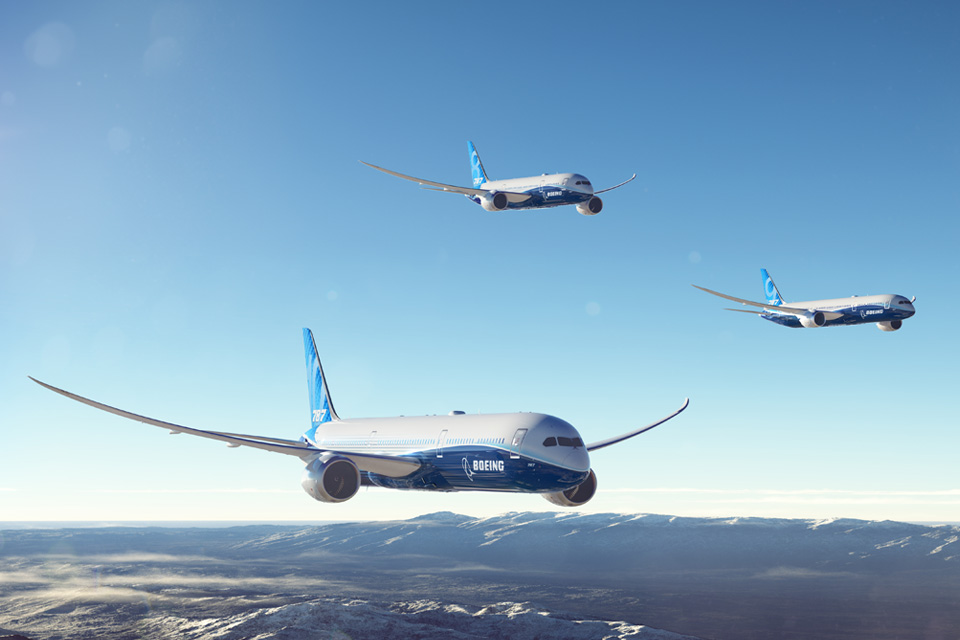
\includegraphics[width=\textwidth]{./figure/787-dreamliner.jpeg}    
    \caption{波音B787,Dreamliner梦想客机}
    \label{fig:B787}
\end{figure}

\begin{lstlisting}
    \begin{figure}[!ht]
        \centering 
        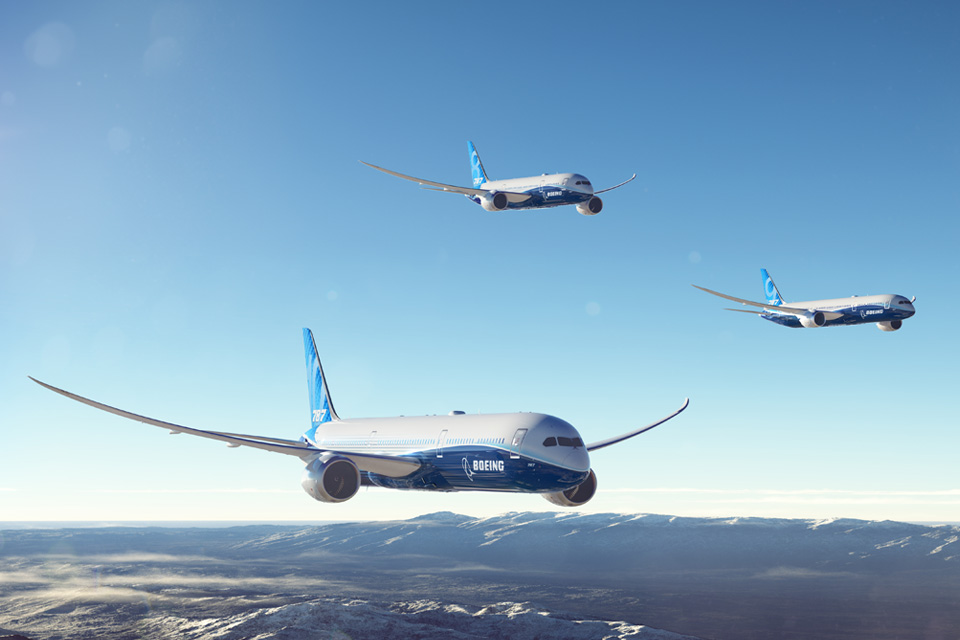
\includegraphics[width=\textwidth]{./figure/787-dreamliner.jpeg}    
        \caption{波音B787,Dreamliner梦想客机} % \caption 必须在 \label之前,否则不能正常交叉引用
        \label{fig:B787}
    \end{figure}   
\end{lstlisting}

也可以插入一些子图,如下\Cref{fig:A350} 
\begin{figure}[!ht]
    \centering 
    \begin{subcaptionblock}{0.48\textwidth}
        \centering 
        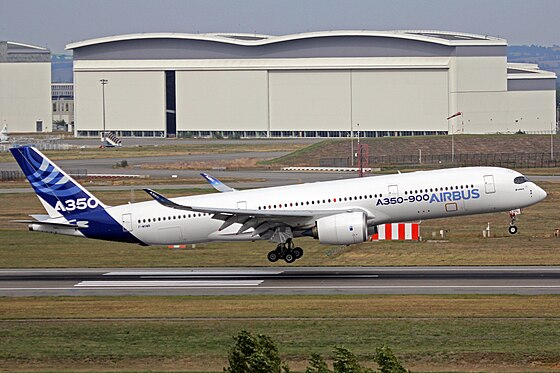
\includegraphics[width=\linewidth]{./figure/A359.jpg}
        \caption{Airbus A350-900}
        \label{fig:A359}
    \end{subcaptionblock}
    \begin{subcaptionblock}{0.48\textwidth}
        \centering
        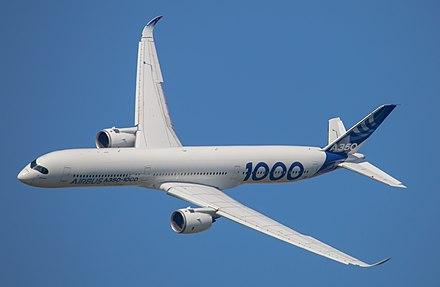
\includegraphics[width=\linewidth]{./figure/A35k.jpg}
        \caption{Airbus A350-1000}
        \label{fig:A35k}
    \end{subcaptionblock}
    \caption{Airbus A350家族}
    \label{fig:A350}
\end{figure}

\begin{lstlisting}
\begin{figure}[!ht]
    \centering 
    \begin{subcaptionblock}{0.48\textwidth}
        \centering 
        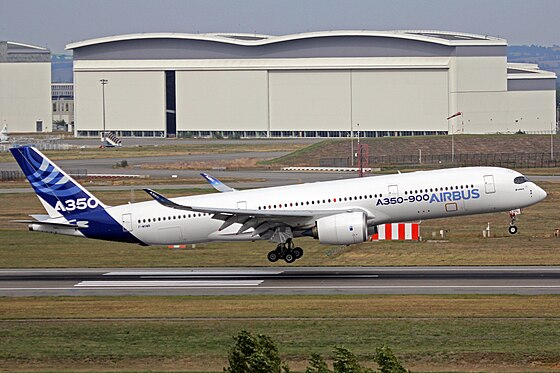
\includegraphics[width=\linewidth]{./figure/A359.jpg}
        \caption{Airbus A350-900}
        \label{fig:A359}
    \end{subcaptionblock}
    \begin{subcaptionblock}{0.48\textwidth}
        \centering
        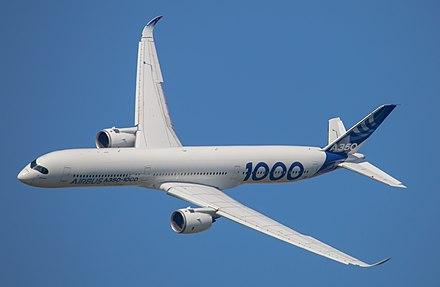
\includegraphics[width=\linewidth]{./figure/A35k.jpg}
        \caption{Airbus A350-1000}
        \label{fig:A35k}
    \end{subcaptionblock}
    \caption{Airbus A350家族}
    \label{fig:A350}
\end{figure} 
\end{lstlisting}

\subsection{表格}
论文一般要求插入三线表,需要在导言区引用宏包{\ttfamily booktabs}
(该宏包已在V0.2.1版本之后,由模板添加,所以不需要在导言区引用)
\begin{lstlisting}
    \usepackage{booktabs}
\end{lstlisting}

比如下\Cref{tab:example}
\begin{table}[!ht]
    \centering 
    \caption{示例表}
    \label{tab:example}
    \setlength{\tabcolsep}{5em}{
    \begin{tabular}{cc}
        \toprule
        项目 & 值\\
        \midrule
        质量(Kg) & 2 \\
        长度(m) & 2 \\ 
        \bottomrule
    \end{tabular}}
\end{table}

\begin{lstlisting}
\begin{table}[!ht]
    \centering 
    \caption{示例表}
    \label{tab:example}
    \setlength{\tabcolsep}{5em}{
    \begin{tabular}{cc}
        \toprule
        项目 & 值\\
        \midrule
        质量(Kg) & 2 \\
        长度(m) & 2 \\ 
        \bottomrule
    \end{tabular}}
\end{table}   
\end{lstlisting}

\thanks
模板提供了致谢环境。
\begin{lstlisting}
    \thanks
\end{lstlisting}

\newpage
\subsection{参考文献}
模板使用参考文献的样式为GB7714-2015,符合论文要求。
通过 {\ttfamily BibLaTeX}管理参考文献,需要指定
{\ttfamily bib}文件\cite{aerospace11060494}
,通过\lstinline|\cite{<name>}|
引用参考文献\cite{FHLX200903002}。
\begin{lstlisting}
    % 指定bib文件,需要放在导言区
    \addbibresource[location=local]{reference.bib}
    
    % 打印参考文献
    % 这句命令必须要添加在 \end{document} 命令之前
    % 以打印参考文献条目,否则将不会打印参考文献
    % 该命令你可以放在任何地方,则会在该命令的当前
    % 打印参考文献的条目
    % NOTE:该命令不可使用两次,以防出现不可预知的
    % 错误,即该命令只能在全文中出现一次
    % 为加快编译速度,建议仅用xelatex编译,最后定稿
    % 时,再使用编译链编译,以生成正确的交叉引用
    \printreference
\end{lstlisting}

注意,要正确编译,产生参考文献,必须要采用如下编译方式:

{\ttfamily xelatex <jobname.tex> -> biber <jobname> -> xelatex 
<jobname.tex> -> xelatex <jobname.tex>}

{\ttfamily bib}后端为 {\ttfamily biber}。
\printreference

\newpage
\appendix

\section{其他设置}
\subsection{附录}
如果你需要添加附录,请在导言区引用{\ttfamily appendix}宏包
\begin{lstlisting}
    \usepackage{appendix}

    % 在需要添加附录的部分添加如下命令
    \newpage % 另起一页
    \appendix 

    % 后面正常按照正文书写即可
    \section{}
\end{lstlisting}

\subsection{代码抄录}
模板没有定制代码抄录环境,需要自行定制样式
\begin{lstlisting}
    % 使用该宏包定制样式
    \usepackage{listings}
\end{lstlisting}

\subsection {节标题分页}
模板默认节标题与上一节内容是相连的,如果想要新的一节另起一页,有如下两个
方法,
\begin{enumerate}
    \item 在新的节标题前面添加命令 \lstinline|\newpage|
    \item 在导言区添加命令 \lstinline|\ctexset{section/break=\clearpage}|
\end{enumerate}
二者任选其一即可。


\end{document}
